\documentclass{article}
\usepackage{indentfirst}
\usepackage{lmodern}
\usepackage[utf8]{inputenc}
\usepackage[T1]{fontenc}
\usepackage[ngerman]{babel}
\usepackage{amssymb,amstext,amsmath}
\usepackage{graphicx}
\usepackage{dsfont}
\usepackage{amsfonts}
\usepackage{graphics}
\usepackage{float}
\usepackage{cite}
\usepackage{url}
\usepackage{tabularx}
\usepackage{capt-of}

\title{Transistor}
\author{Alexander Heinisch, Dominik Wille}
\begin{document}
\maketitle
\begin{center}
\begin{minipage}{\linewidth}
\centering
\makebox[0cm]{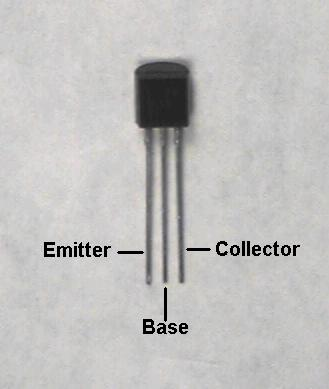
\includegraphics[width=8cm]{bilder/tra7}}
\label{ringe}
\end{minipage}
\end{center}
\vspace{3cm}
\noindent
\begin{center}
\begin{tabular}{r l}
Tutor & Sebastian Baum  \\
Durchführung & 22. Mai 2013 von 14-18 Uhr \\

E-Mail Dominik & dominik.wille@fu-berlin.de \\
E-Mail Alexander & matthias.heinisch@gmx.de \\
\end{tabular}
\end{center}

\newpage
\tableofcontents
\newpage

\section{Physikalische Grundlagen}
Ein Transistor (aus dem engl. transfer resistor) ist ein elektronisches Bauelement, welches zum
schalten und verstärken von elektrischen Signalen benutzt wird. Er besteht aus einer dreifachen
Halbleiterschichtfolge (p-n-p oder n-p-n). Da ein p-n-Übergang einer Diode entspricht kann man den 
Transistor als zwei dieser Dioden, die entgegengesetzt geschaltet sind sehen. Die Elektroden des
Transistors heißen Emitter, Basis und Kollektor (siehe Abbildung \ref{transistor}). Um die 
Funktionsweise des Transistor besser zu verstehen, wird zunächst näher auf die Halbleiter 
eingegangen.

\subsection{Das Bändermodell}
Um Prozesse in Halbleiten erklären zu können bietet es sich an quantenmechanische Effekte im Festkörper in ein neues Modell, das so genannte Bändermodell zu überführen.

Da in einem Festkörper grundsätzlich eine große Anzahl von Atomen vorhanden ist reicht es nicht aus ein einzelnes Atom zu betrachten. Im Atom außenliegende Elektronen sind im Festkörper nicht an einzelne Atome gebunden sondern wandern durch die überlappenden Wellenfunktionen benachbarter Atome durch den gesamten Festkörper. Die Gesamtheit eines solchen Zustands bezeichnet man als {\it Band}.
Diese Bänder erstrecken sich demnach über den Gesamten Festkörper. 

\subsection{Halbleiter}
Halbleiter sind, je nach dem welche Temperatur in ihnen herrscht sie haben, Leiter oder Isolatoren. Im allgemeinen verbessert sich die Leitfähigkeit mit steigender Temperatur. Die Leitfähigkeit am absoluten Temperaturnullpunkt von 0 K ist nahezu Null. 
Das liegt daran, dass sich durch thermische Anregungen Elektronen von den Atomen lösen und somit 
Lücken in den Leitungsbändern (die oberste teilbesetzte bzw. leere Schicht der Atomhülle) 
entstehen. Die 
Schicht darunter bezeichnet man als Valenzband und ist durch eine ''verbotene Zone'' von dem 
Leitungsband getrennt. Demnach sind die Elektronen dieser beiden Bänder {\it quasifrei} im 
Festkörper, während die Elektronen darunter an ihren Kern gebunden sind (Atomrümpfe als Ionen). 
Im Vergleich dazu wird in der Folgenden Grafik der Unterschied zwischen Leiter, 
Halbleiter und Isolatoren in Bezug 
auf die ''verbotene Zone'' dargestellt.
\begin{center}
\begin{minipage}{\linewidth}
\centering
\makebox[0cm]{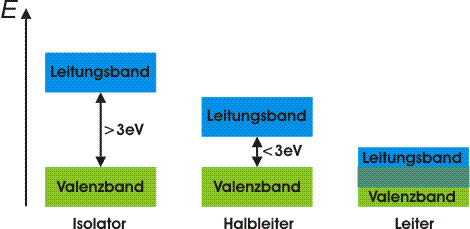
\includegraphics[width=\textwidth]{bilder/tra2}}
\captionof{figure}{Unterschied zwischen Leiter, Halbleiter und Isolatoren}%
\label{halbleiter}
\end{minipage}
\end{center}

Wie man sieht, ist bei Isolatoren die ''verbotene Zone'' ziemlich groß und bei Raumtemperatur können keine Elektronen diese Zone passieren. Bei Halbleitern hingegen wird bei Raumtemperatur schon ein kleiner Teil der Elektronen in das Leitungsband bringen.

\subsection{Eigenleitung}
Der Übergang der Elektronen von dem Valenzband zum Leitungsband wird über die Boltzmannverteilung für thermische Anregungen beschrieben. Die daraus berechenbare Leitfähigkeit eines Halbleiters wird als Eigenleitung bezeichnet. Jedes Elektron des Leitungsbandes hinterlässt eine Lücke im Valenzband (''Defektelekronen''), wobei die Dichte n der quasifreien Elektronen und die Anzahl p der Lücken sind gleich groß.\\
Man erhält damit in Abhängigkeit der Temperatur folgende Gleichung:
\begin{equation}
n(T)\ \text{bzw.}\ p(T) \propto T^{\frac{3}{2}}\cdot e^{-\frac{\Delta E}{2kT}}
\end{equation}

mit \(\Delta E\) als Abstand zwischen Valenz- und Leitungsband.

\subsection{Störstellenleitung}
Nun kann man sogenannte Störstellenhalbleiter bauen. Dabei wird ein fünfwertiges Fremdatom (mit fünf freie Elektronen) in ein vierwertiges Kristallgitter gesetzt, wodurch dieses fünfte überschüssige Elektron nicht durch Nachbaratome gebunden wird. Das hat zur Folge, dass schon Raumtemperatur reicht, um das Elektron zu lösen und in einen Energiezustand dicht unterhalb des Leitungsbandes zu heben (n-Halbleiter). Im Falle eines dreiwertigen Fremdatoms wird die Fehlstelle bei einer thermischen Anregung (bei Raumtemperatur) besetzt, womit ein Defektelektron im Valenzband als quasifreier positiver Ladungsträger übrig bleibt (p-Halbleiter).

\subsection{p-n-Grenzschicht}
Befinden sich nun eine p- und eine n-Schicht in direktem Kontakt, so diffundieren Löcher und Elektronen wegen den thermischen Bewegungen in die jeweils entgegengesetzt polarisierten Gebiete. Durch diese ''Wanderungen'' werden die Atome an der Grenzzone neutralisiert und der Rest der Schicht wird polarisiert, was wiederum ein elektrisches Feld erzeugt welches der Diffusion entgegen wirkt.
\begin{figure}[H]
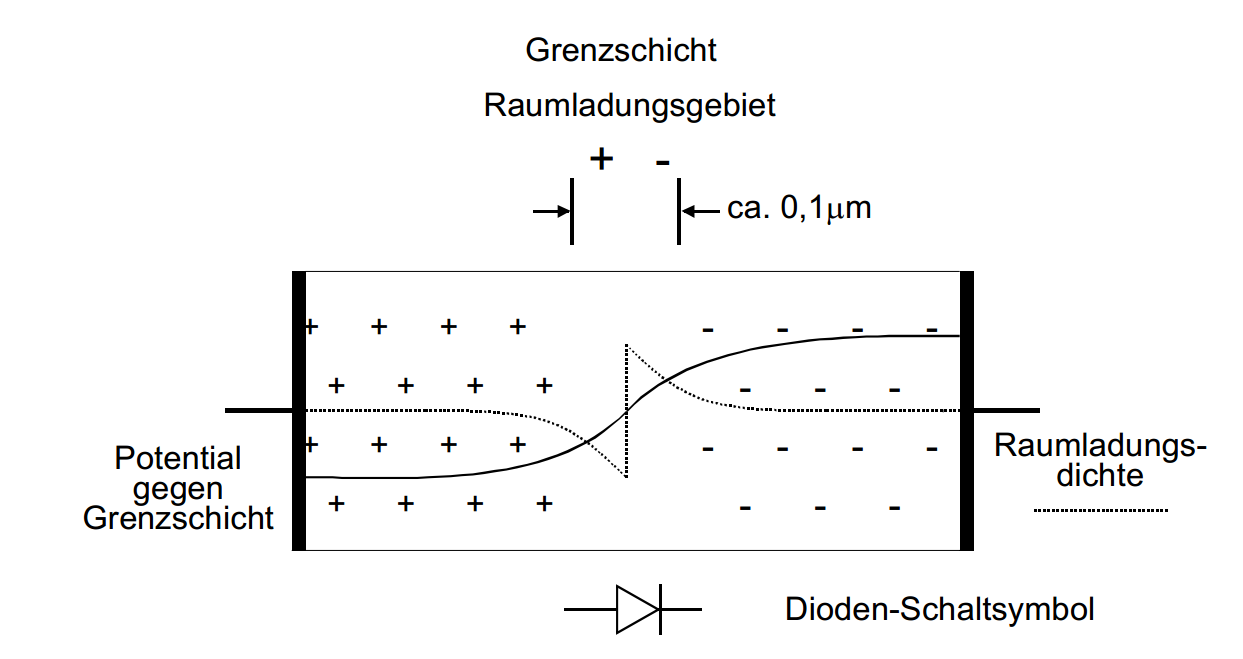
\includegraphics[width=\textwidth]{bilder/tra3}
\caption{p-n-Grenzschicht und Halbleiterdiode}
\end{figure}

Die Rekombination der Atome in der Grenzzone erzeugt eine hochohmige Sperrschicht. Je nach Polarisation wird durch Anlegen einer äußeren Spannung die Sperrschicht durch einen Ladungsträgermangel verbreitert bzw. durch einen Ladungsträgerüberschuss verringert (Sperrichtung und Durchlassrichtung). Der Stromfluss wird also nur in eine Richtung zugelassen

\subsection{Halbleiterdiode}
Nun kommt es drauf an, wie die äußere Spannung gepolt ist. Wenn man die äußere Spannung mit (+) an n und (-) an p anlegt, verbreitert sich die Sperrschicht, da Ladungsträger aus den Gebieten abgezogen werden (Sperrichtung). Polt man ihn nun um, wird die Sperrschicht abgebaut und die Diode ist in Flussrichtung geschaltet.\\
Mittels der sogenannten Shockley-Diodengleichung kann man den Strom in Abhängigkeit der äußeren Spannung die Kennlinie der Diode berechnen:
\begin{equation}
I=I_s \left(e^{\frac{e}{kT}U}-1\right)
\end{equation}

\(I_s\) ist der praktisch konstante Strom in Sperrichtung und der Exponent ist die Temperaturspannung. Si oder GaAs Kennlinien weichen u.a. von dieser Gleichung ab und zeigen erst ab einer bestimmten Schwellspannung ein Durchschalten in Flussrichtung.

\subsection{Transistor}
Wie schon zuvor erwähnt, besteht ein Transistor aus drei Halbleiterschichten, also aus zwei entgegengesetzt geschaltete Halbleiterdioden. Legt man nun bei einem npn-Transistor eine äußere Spannung mit (-) an den Emitter und mit (+) an den Kollektor an, wird kein Strom fließen. Der Transistor ist im Basis-Kollektor-Übergang in Sperrichtung geschaltet. Wenn an die Basis ebenfalls eine (+) Spannung angelegt wird, wird die Emitter-Basis Diode auf Durchlassrichtung geschaltet, wodurch Elektronen aus dem Emitter in den Basisbereich eintreten können.\\
Es können Trasistoren so gebaut werden, dass fast 100\(\%\) der Elektronen in den Kollektorkreis gelangen, wodurch ein relativ kleiner Basis-Steuerstrom einen großen Kollektor-Laststrom regeln kann (Verstärkerfunktion des Transistors).

\begin{center}
\begin{minipage}{\linewidth}
\centering
\makebox[0cm]{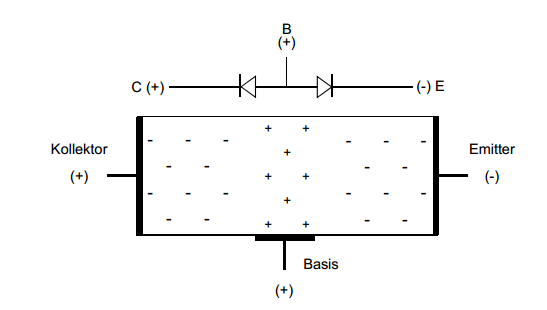
\includegraphics[width=\textwidth]{bilder/tra1}}
\captionof{figure}{Aufbau eines npn-Transistors}%
\label{transistor}
\end{minipage}
\end{center}

\subsection{Kenngrößen und Kennlinienfelder}
Beschreiben kann man einen Transistor durch drei Ströme und drei Spannungen: \(I_B,I_C,I_E\) und \(U_{EC},U_{BC},U_{EB}\)
Es gilt:
\begin{equation}
I_B+I_C+I_E=0
\end{equation}

Dabei sind hineinfließende Ströme positiv und herausfließende Ströme negativ.\\
Des weiteren gilt für die Spannungen
\begin{equation}
U_{EC}=U_{BC}+U_{EB}
\end{equation}

Somit sind immer vier der sechs Variablen frei wählbar.
Ist der Transistor in Emitterschaltung, so kann man ihn als Stromverstärker auffassen. In einem Vier-Quadranten-Kennlinienfeld wird die Abhängigkeit der vier Variablen dargestellt\\

Das Kennlienenfeld beinhaltete in diesen Quadranten folgende Inhalte:\\
\begin{itemize}
\item 1. Quadrant: Ausgangswiderstand ($U_{EC}$ über $I_C$) mit Arbeitswiderstand $R_A = \frac{-1}{m}$ (fallende Gerade mit Steigung m)
\item 2.Quadrant: Stromverstärkung $\beta  (I_C$ über$ I_B)$
\item 3.Quadrant: Eingangswiderstand $(U_{EB} $über$ I_B)$
\item 4.Quadrant: Spannungsrückwirkung $(U_{EB}$ über$ U_{EC})$ 
\end{itemize}

\begin{center}
\begin{minipage}{\linewidth}
\centering
\makebox[0cm]{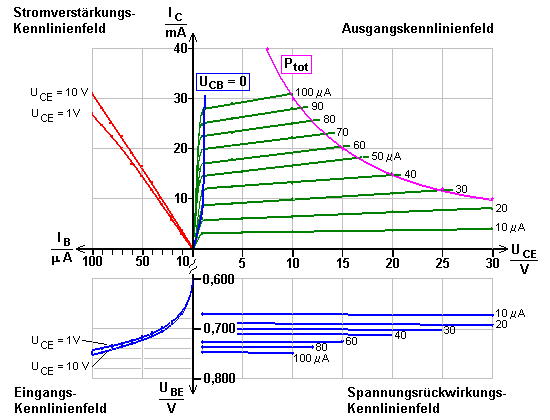
\includegraphics[width=\textwidth]{bilder/tra4}}
\captionof{figure}{Vier-Quadranten-Kennlinien}%
\label{kennlinienfeld}
\end{minipage}
\end{center}

Hier sieht man im ersten Quadrant, dass der Kollektorstrom nur geringfügig von der Emitter-Kollektor-Spannung abhängt. Das hat zur Folge, dass ein Spannungsabfall am Verbraucher nur zu einer geringen Gegensteuerung der Verstärkung führt.\\
Der zweite Quadrant gibt Auskunft über die Stromverstärkung, welche den folgenden Relationen folgt:
\begin{equation}
\beta =\frac{I_C}{I_B}\ \text{bzw.}\ =\frac{\Delta I_C}{\Delta I_B}
\end{equation}

Im dritten Quadrant wird eine ''normale'' Diodenkennlinie in Flussrichtung veranschaulicht, in diesem Fall ist es die Emitter-Basis-Diode.\\

Im letzten Quadrant wird veranschaulicht den Zusammenhang zwischen Emitter-Kollektor-Spannung und der Basisspannung.

\subsection{Spannungsverstärkung}
Durch einen Arbeitswiderstand \(R_A\) lässt sich der Kollektorstrom begrenzen und die Emitterschaltung stellt einen einfachen Spannungsverstärker dar. Die durch \(R_A\) verursachte Spannungsänderung ist dabei proportional zu der Stromänderung.
Das Verhältnis der Spannungsverstärkung v wird dabei beschrieben durch:
\begin{equation}
v=\frac{\Delta U_{EC}}{\Delta U_{EB}}=\frac{R_A \cdot \Delta I_C}{\Delta U_{EB}} \vline \cdot\frac{\Delta I_B}{\Delta I_B} =\frac{\beta \cdot R_A}{r_{EB}}
\end{equation} 

Dabei ist \(r_EB\) der differentielle Eingangswiderstand \(\Delta U_{EB}/\Delta I_B\).

\subsection{Arbeitspunkt}
Da ein Transistor nur im Bereich positiver Emitter-Basis-Ströme verstärkt, muss die Basis mit positivem Gleichstrom überlagert werden, um Wechselstromsignale unverzerrt weiterleiten zu können. Die wird durch den sogenannten ''Arbeitspunkt'' in den Kennlinienfeldern dargestellt. Man nimmt für ihn die halben maximal zulässigen Kollektorströme bzw. die halben Versorgungspannungen.

\subsection{Stabilisierung}

Die Leitfähigkeit von Halbleitern hängt wie schon zuvor erwähnt, stark von der Temperatur ab, wodurch die Eigen- und Fremderwärmung ebenfalls einen Einfluss darauf hat. Um dem entgegenzuwirken, werden verschiedene Stabilisierungsmethoden eingebaut. Eine der wichtigsten ist die sogenannte Gegenkopplung, bei welcher ein Teil des verstärkten Ausgangssignals invertiert auf den Eingang zurück geführt wird, was wiederum einen Verlust der Gesamtverstärkung verursacht.\\
Wir wollen eine Parallelgegenkopplung untersuchen. Dabei wird das Maß der Stabilisierung durch die Rückkopplungswirkung \(\alpha=frac{\Delta U_{EB}}{\Delta U_{EC}}\) und die Spannungsverstärkung v beschrieben. Nehmen wir nun an, dass \(\Delta U_{EC}\)' eine Kollektorpotentialänderung ohne Gegenkopplung ist, dann gilt:

\begin{equation}
\Delta U_{EC}=U_{EC}'-\alpha U_{EC}\cdot v
\end{equation}
Die nun nach der tatsächlichen Spannungsänderung aufgelöst, ergibt:

\begin{equation}
U_{EC}=\frac{U_{EC}'}{1+\alpha \cdot v}
\end{equation}
\(\Rightarrow\) je größer der Rückkopplungsfaktor und die Verstärkung desto kleiner ist die tatsächliche Ausgangsspannungsschwankung.
\newpage
\section{Aufgabenstellung}
\subsection*{Aufgabe 1}
Aufnahme und Konstruktion des (statischen) Kennlinienfeldes eines npn-Transistors für eine
angenommene Betriebsspannung (Versorgungsspannung) von 12 V. Bestimmung der Stromverstärkung für
den statischen Fall. Aufbau einer Verstärkerstufe mit einer Parallel- Gegenkopplung zur
Stabilisierung.

\subsection*{Aufgabe 2}
\subsubsection*{Aufgabe 2.1}
Dimensionierung der Schaltung: Abschätzung des Arbeitswiderstandes und des Basisvorwiderstandes.
\subsubsection*{Aufgabe 2.2}
Experimentelle Überprüfung der Kollektor-Widerstandsgeraden durch Variation des
Basisvorwiderstandes und Bestimmung der Stromverstärkung.
\subsubsection*{Aufgabe 2.3}
Verstärkung einer Eingangs-Wechselspannung als Signal. Messung der Spannungsverstärkung und Vergleich mit der theoretischen Erwartung.

\newpage

\section{Aufgabe 1}
\begin{center}
\begin{minipage}{\linewidth}
\centering
\makebox[0cm]{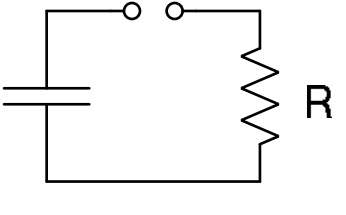
\includegraphics[scale=0.5]{sb1}}
\captionof{figure}{Schaltplan Aufgabe 1}%
\label{schaltplan_nr1}
\end{minipage}
\end{center}

Für diese Aufgabe haben wir einen Kondensator mit einem Widerstand in Reihe geschalten (siehe Abbildung 1.1). Mit einem Frequenzgenerator legten wir eine Spannung an und mit Hilfe eines Oszilloskops veränderten wir die Frequenz, bis beide Sinuskurven die gleiche Spannung hatten. 
Damit die Teilspannung an der Spule und am Kondensator übereinstimmen muss folgendes gelten:
\begin{equation}
U_C = U_R 	\Rightarrow	 U_{ges} = U_C + U_R
\end{equation}
Mit einem Spannungsmessgerät (Fluke 175) haben wir die Spannung zwischen dem Widerstand und dem Kondensator gemessen. Dabei betrug der Spannungsunterschied:
\begin{equation}
\notag
\Delta U=0,023 V
\end{equation}

Die Frequenz betrug dabei konstant:

\begin{equation}\notag
f_{char} = (160,45\pm 0,1) Hz
\end{equation}

Die verwendeten Bauteile des R-C-Kreises wurden separat noch einmal nachgemessen, dabei ergab sich für den Widerstand einen Wert von:
\begin{equation}\notag
R = (0.990 \pm 0.012)k\Omega
\end{equation}

und die Kapazität des Kondensators:
\begin{equation}\notag
C = (1.001 \pm 0.013)\mu F
\end{equation}

Die Fehler errechnen sich aus $\pm (1.0\% +3dgt)$.

\subsection{Berechnung der Frequenz}
Nun können wir über folgende Formel den theoretischen Wert der Frequenz f berechnen:
\begin{equation}\notag
f_{theo}=\frac{1}{2\pi RC}= (160.6 \pm 2.0)Hz
\end{equation}

Den Fehler bestimmen wir über die Gauß'sche Fehlerfortpflanzung:
\begin{equation}\notag
\Delta f_{theo}=\sqrt{\left(\frac{\partial f_{theo}}{\partial R}\cdot \Delta R\right)^2+\left(\frac{\partial f_{theo}}{\partial C}\cdot \Delta C\right)^2}
\end{equation}

\subsection{Phasenverschiebung}
Für die Phasenverschiebung haben wir bei einer Frequenz von f = 160,30 HZ am Oszilloskop ein \(\Delta\)t = 0,8ms abgelesen. Dafür ergibt sich für \(\phi\) einen Wert für:
\begin{equation}
\notag
\phi = 2\pi f \Delta t = (0,806 \pm 0,009)^\circ = (0,257\pm 0,003)\pi
\end{equation}

Somit ergibt sich wie erwartet \(\frac{\pi}{4}\) für die Phasenverschiebung.
Um nun noch die Phasenverschiebung auszurechnen, benutzten wir:
\begin{equation}\notag
\phi_{theo}=arctan\left(\frac{1}{\omega RC}\right)=\left(0,7854 \pm 0.0065\right)^\circ =(0,250\pm 0,003)\pi
\end{equation}

Den Fehler bekommen wir aus:
\begin{equation}\notag
\Delta \phi_{theo}=\sqrt{\left(\frac{\partial \phi_{theo}}{\partial f_{theo}}\cdot \Delta f_{theo}\right)^2+\left(\frac{\partial \phi_{theo}}{\partial C}\cdot \Delta C\right)^2+\left(\frac{\partial \phi_{theo}}{\partial R}\cdot \Delta R\right)^2}
\end{equation}

\subsection*{Fazit}
Den Wert für die charakteristische Frequenz konnten wir relativ schnell finden, nachdem wir festgestellt hatten, dass ein Messgerät einen Wackelkontakt hatte und bis dahin nur seltsame Werte geliefert wurden.\\
Der theoretische und der gemessene Wert der charakteristische Frequenz sind gleich, nur dass der Fehler des theoretischen Werts aufgrund der Bauteile doch relativ groß ist. Die Phasenverschiebung ist auch ziemlich klein.

\section{Aufgabe 2}
\subsection{Abschätzung des Arbeitswiderstandes}

Um den Arbeitswiderstand zu bestimmen, benutzen wir das Vier-Quadranten-Kennlinienfeld (Abbildung 7) und gehen vom äußersten Punkt des dritten Quadranten für \(I_B\)= 140,8\(\mu A\) senkrecht nach oben. Im Zweiten Quadranten treffen wir so den Wert für \(I_C\)=13,9 mA, welches unser Startpunkt der Arbeitsgeraden (bzw. Kollektor-Widerstandsgerade) sein wird. Damit ergeben sich die Koordinaten (\(U_{CE}\) = 0[V], \(I_{C}\) = 13,9[mA]) für den Punkt \(P_1\) des Kurzschlussfalls. Der Punkt \(P_2\) liegt bei den Koordinaten (\(I_{C}\) = 0 [mA],\(U_{CE}\) = 12[V]), weil 12[V] die maximale Versorgungsspannung betrug.\\
Der Arbeitspunkt \(P_{A}\) liegt laut Definition bei \(\left(\frac{U_{CE}}{2}, \frac{I_{C}}{2}\right)\), welches bei uns den Werten (6.055[V],6.95[mA]) entspricht.\\

Den Arbeitswiderstand wird über die Formel:
\begin{equation}
\notag
R_{A}=\mid \frac{1}{m}\mid = \left(\frac{U_{EC}}{I_C}\right) = 871.23 \Omega
\end{equation}\\

Während des Versuchs haben wir für den Arbeitswiderstand einen Wert von (\(464.3\pm 2.6)\Omega\) gemessen.\\

Der Basisvorwiderstand ergibt sich aus der Formel:
\begin{equation}
\notag
R_V= \frac{U_{EC}-U_{EB}}{I_B}=\frac{6V-0.7V}{(63.5\cdot 10^{-6})A}=83.5k\Omega
\end{equation}

Hier hatten wir einen Wert von (\(100.2\pm 0.8)k\Omega\) gemessen. Auf die Unterschiede dieser Werte werden wir später in der Diskussion eingehen.

\subsection{Überprüfung der Kollektor-Widerstandsgeraden}

Nun überprüfen wir die abgeschätzten Werte, indem wir einen Arbeitswiderstand und einen Basisvorwiderstand in die Schaltung einbauen (siehe Abbildung 6) und eine neue Messreihe aufnehmen. Wir steigern dabei die Werte für \(I_B\) in gleichen Abständen und notieren, wie sich die anderen Größen dazu verhalten. \(U_0\) hielten wir konstant auf (\(12.11\pm 0.09\))

\newpage
Unsere Messung ergaben folgende Werte:\\

\begin{center}
\begin{tabular}{r r r r}
\(I_B [\mu A]\) & \(I_C [mA]\) & \(U_B [V]\) & \(U_{CE}[V]\) \\
\hline
\(52.116\) & \(9.0\) & \(0.116\) & \(7.93\) \\ 
\(62.519\) & \(9.3\) & \(0.191\) & \(7.75\) \\ 
\(72.518\) & \(9.7\) & \(0.255\) & \(7.59\) \\ 
\(81.305\) & \(10.0\) & \(0.315\) & \(7.45\) \\ 
\(94.132\) & \(10.5\) & \(0.362\) & \(7.22\) \\ 
\(101.505\) & \(10.9\) & \(0.429\) & \(7.01\) \\ 
\(113.423\) & \(11.8\) & \(0.526\) & \(6.61\) \\ 
\(122.311\) & \(12.6\) & \(0.586\) & \(6.24\) \\ 
\(131.906\) & \(22.7\) & \(0.755\) & \(1.52\) \\ 
\(142.410\) & \(23.4\) & \(0.757\) & \(1.17\)
\end{tabular}
\captionof{table}{Rohmesswerte für Aufgabe 2.2}
\end{center}


\newpage
\section{Fazit}
In der ersten Aufgabe sollten wir ein Vier-Quadranten-Kennlinienfeld eines npn-Transistors erstellen. Dazu nahmen wir die Größen \(I_B, I_C, U_{EC},\) und \(U_{Be}\) auf. Nachdem ein Messgerät Werte im vollkommen falschen Messbereich ausgab, eine Fehlersuche erfolglos blieb, die Schaltung nochmal neu aufgebaut wurde und wir dadurch sehr viel Zeit verloren hatten, wechselten wir das Messgerät aus und erhielten nun Messwerte im richtigen Messbereich. Durch den Zeitverlust entschlossen wir uns, die aufgenommenen Werte nicht sofort auf das Millimeterpapier zu übertragen. Während der Messung selber fiel mal das eine Messgerät aus weil die Batterie leer war und ein anderes Messgerät schaltete sich ohne ersichtlichen Grund von selbst ab. Auch hatte das etwas veraltete Steckbrett ein paar Wackelkontakte, durch welche wohl einige Sprünge in unseren Messwerten erklärt werden können.\\
Des weiteren können wir zusammenfassend zum Kennlinienfeld sagen:
\begin{itemize}
\item Die Werte im ersten Quadranten entsprachen nicht denen der theoretischen Vorlage
\item Die Werte des zweiten Quadranten liefern nur unsichere Ergebnisse. Da wir nur vier Spannungen gemessen hatten und demnach nur vier Werte aufnehmen konnten, können wir nichts mit Sicherheit Bestätigen oder Widerlegen.
\item Auch im dritten Quadranten haben wir nur vier Messwerte und können nichts genaueres über die Qualität der Messung sagen.
\item Die Werte des vierten Quadranten scheinen ganz gut zu sein. Nur dass der Sprung in der 30\(\mu A\) Linie auf das Austauschen des Messgeräts zurückzuführen ist.
\end{itemize}

In Aufgabe 2 sah es nicht besser aus. Der geschätzte Wert für den Arbeitswiderstand ist mir \(871,23\Omega\) fast doppelt so groß wie der gemessene Wert von \(464,3\Omega\). Bei dem Basisvorwiderstand erhielten wir einen geschätzten Wert von \(83,5k\Omega\), welcher sich ebenfalls von den gemessenen \(100,2k\Omega\) stark unterscheidet.\\

Bei der Überprüfung der Kollektor-Widerstandsgeraden bauten wir die Schaltung geringfügig um und nahmen erneut Werte für die vier vorher aufgezählten Größen auf. Dabei steigerten wir \(I_B\) jeweils um etwa 10\(\mu A\). Auffällig ist auch hier, dass sich die jeweils letzten beiden Werte für \(I_C, U_{EC},\) und \(U_{Be}\) von den anderen stark unterscheiden. In Abbildung 8 sehen die Ergebnisse sehr vielversprechend aus. In Abbildung 9 hingegen ist klar erkennbar, dass auch hier die alten bekannten Probleme mit Wackelkontakten etc. seltsame Werte verursachten.\\

Zusammenfassend ist zu sagen, dass der Versuch allem Anschein nach nicht erfolgreich gewesen ist. Wackelkontakte und defekte Messgeräte sind soweit wir das beurteilen konnten, die Ursache. Damit haben wir zwar kleine statistische Fehler aber große systematische Fehler.

\section{Quellenangabe}
\begin{itemize}
\item GPII-Skript
\item Platzskript
\item Abbildung 4: \(http://141.7.70.48/images/theory_abb5.gif\)
\item Abbildung 6: \(http://elektroniktutor.de/bauteilkunde/bt_pict/trkennl.gif\)
\end{itemize}
\vspace{7.0cm}

\begin{tabularx}{\textwidth}[b]{p{5cm} X p{5cm}} \cline{1-1} \cline{3-3}
Datum, Dominik Wille & & Datum, Alexander Heinisch
\end{tabularx}
\end{document}
